%% JAIR Manuscript (acmart) - Clement Frassier
%% Federated Learning: Principles and Implementation
%% Nurse Stress Detection (HEART Project)
%% English translation of the condensed version (rapport_reduit_15p.tex)

\documentclass{acmart}
\usepackage{amsmath, amssymb}
\usepackage{booktabs}
\usepackage{graphicx}
\usepackage{hyperref}
\usepackage{xcolor}
\usepackage{enumitem}
\setlist{itemsep=2pt, topsep=3pt}

%\setcopyright{cc}
%\acmDOI{10.1613/jair.1.xxxxx}

%\JAIRAE{Clement Frassier}
%\JAIRTrack{Applications}
%\acmVolume{4}
%\acmArticle{6}
%\acmMonth{8}
%\acmYear{2026}

\RequirePackage[
  datamodel=acmdatamodel,
  style=numeric,
  backend=biber,
  giveninits=true,
  uniquename=init
  ]{biblatex}

\renewcommand*{\bibopenbracket}{(}
\renewcommand*{\bibclosebracket}{)}

\addbibresource{sample-base.bib}

\begin{document}

\title[Extreme Heterogeneity in FL: Centralized Collapses Too]{When Heterogeneity Makes Even the Centralized Model Collapse: A Federated Learning Case Study for Nurse Stress Detection \\ \large Condensed Version}

\author{Clement Frassier}
\orcid{0009-0000-0000-0000}
\email{clement.frassier@gmail.com}
\affiliation{%
  \institution{UKM / UEL}
  \city{Kuala Lumpur}
  \country{Malaysia}
}

\begin{abstract}
{\bf Background:}
Physiological data collected via connected wristbands in hospital settings constitute
personal health data subject to the GDPR~\cite{gdpr2016}. Aggregating them on a
central server exposes patients and staff to major re-identification risks, making
classic centralized approaches unsuitable in this context.

{\bf Objectives:}
We aim to train an automatic stress-detection model on data distributed across 15
nurses, without ever transmitting this data to a central server, while providing a
formal differential-privacy guarantee and producing a model deployable on an embedded
wristband (TinyML).

{\bf Methods:}
We propose a federated learning pipeline combining FedProx ($\mu = 0{,}05$) for
Non-IID heterogeneity, and DP-SGD via Opacus for $(\varepsilon, \delta)$-DP
differential privacy. The MLP Tiny model (1~362 parameters, 5.32~KB) is trained over
30 communication rounds and dynamically quantized to INT8 for deployment. A grid
search over 25 federated runs (5 values of $\sigma \in [0.6,\, 1.8]$, 5 independent
seeds) empirically measures the privacy/utility trade-off, compared against an
unconstrained centralized baseline (same model, same 5 seeds, no FL, no DP) that
serves as a theoretical reference ceiling, not deployable in practice on this type of
health data under the GDPR, but useful for honestly quantifying the cost of privacy.

{\bf Results:}
On a pooled test set (all nurses combined), the federated model reaches an accuracy
of $82.0 \pm 0.5\,\%$ on average over the 5 values of $\sigma$, versus
$81.95 \pm 0.89\,\%$ for the centralized model: statistically indistinguishable raw
accuracies. On class-balanced metrics, the centralized model retains an apparent
advantage ($57.8 \pm 1.2\,\%$ balanced-accuracy versus $\approx 47.9\,\%$ for FL). But
11 of the 15 nurses have a single-class test set, where a constant prediction
mechanically achieves $100\,\%$: these clients dominate the pooled result and mask its
true meaning. Restricted to the 4 clients with a genuinely mixed test set, the most
clinically honest measure, the gap shrinks sharply ($45.7 \pm 1.5\,\%$ for the
centralized model versus $42.7 \pm 1.0\,\%$ for FL), and \textbf{the centralized model
itself collapses}: its AUC-ROC drops to $0.267$ (below chance level), and its optimal
decision threshold collapses onto the constant prediction, exactly the same
signature of an absence of generalizable signal previously attributed to FL alone in
a naive pooled evaluation. An ablation of FedProx without DP-SGD confirms that
federation (not privacy) explains most of the residual gap, with privacy adding a
measurable but secondary cost, more visible on these difficult clients ($45.2\,\%$
without DP versus $42.7\,\%$ with DP) than on the pooled metric. Two personalization
architectures (FedPer, then a combination of a multi-layer head, DP restricted to the
extractor, and SCAFFOLD, this last one explored \emph{outside the TinyML size
constraint}, as an upper-bound comparison rather than a deployment target) reduce this
gap statistically significantly on the difficult clients ($48.4\,\%$ then $59.9\,\%$
balanced-accuracy) without eliminating it. Notably, a simple post-hoc fine-tuning of
only the classification head on the already-trained standard FedProx+DP model
($55.9\,\%$) surpasses even FedPer, with no dedicated architecture and no deployment
overhead: the most directly actionable result of this work for real deployment,
which itself remains entirely within the TinyML envelope.

{\bf Conclusions:}
The central result of this work is not that FL is costly compared to the centralized
model, but that \textbf{extreme heterogeneity across nurses limits the generalization
of every architecture tested}, centralized included: on the clients with the most
atypical physiological profile, even a model trained with no privacy or
decentralization constraint whatsoever fails to produce an exploitable signal. FL adds
only a marginal, but real and measurable, disadvantage on top of this underlying
problem. This reframes the research question: it is not about deciding between FL and
centralized training on accuracy (the centralized approach remaining legally
unsuitable for this type of health data under the GDPR regardless, which makes FL the
only viable approach in practice), but about understanding why extreme Non-IID
heterogeneity breaks generalization, and how architectural personalization (FedPer,
SCAFFOLD) can reduce it. Our results honestly quantify this residual cost, show that
it remains stable regardless of the targeted privacy level, and that it can be
significantly mitigated by a personalized architecture, all while keeping a model
deployable on a microcontroller (5.32~KB).
\end{abstract}

\received{20 May 2026}
\received[accepted]{1 July 2026}

\maketitle

\section{Introduction}

Federated Learning (FL) trains a collaborative model without clients' local data ever
leaving their device~\cite{mcmahan2017communication}, a direct response to the data
minimization requirements of the GDPR (Art.~5)~\cite{gdpr2016} and HIPAA~\cite{hipaa1996}
in a medical context. This work is grounded in a use case from the HEART
project\footnote{Health, Engineering, AI, Responsibility and TinyML, a collaboration
between UKM and the University of East London.}: the automatic detection of stress in
15 hospital nurses from physiological signals (connected wristband).

This work starts from a comparison question (can FL approach a centralized model?) but
arrives at a more fundamental result: \textbf{extreme physiological heterogeneity
across nurses limits the generalization of every architecture tested, centralized
included} (Section~\ref{sec:discussion}). On the clients with the most atypical
profile, even a model with no privacy or decentralization constraint whatsoever fails
to produce an exploitable signal. This shifts the research question: no longer a
matter of deciding between FL and centralized training on accuracy, but of
understanding why Non-IID heterogeneity breaks generalization, and to what extent
architectural personalization (FedPer, SCAFFOLD) can reduce it.

\paragraph{Positioning.} FedAvg~\cite{mcmahan2017communication} assumes near-IID
client data; FedProx~\cite{li2020fedprox} relaxes this assumption via a proximal term
but typically evaluates its gain on \emph{simulated} heterogeneity (synthetic
Dirichlet partitions). The FL personalization literature (FedPer~\cite{arivazhagan2019federated},
and drift-correction mechanisms such as SCAFFOLD~\cite{karimireddy2020scaffold})
generally demonstrates a personalization gain \emph{relative} to the federated global
model, without confronting it against a centralized ceiling on the same real-world
heterogeneity. This work's empirical contribution sits precisely there: on a dataset
with \emph{natural}, extreme heterogeneity (individual physiology, not a synthetic
partition), we show that the centralized ceiling itself collapses on the most atypical
clients, an angle less documented in this literature, which most often compares FL to
a centralized model implicitly assumed to be reliable.

\section{Methodology}
\label{sec:method}

\paragraph{FL cycle.} At each round $t$, the server broadcasts the current global
weights $\mathbf{w}^{(t)}$; each client trains locally then returns its updated
weights, aggregated via a partition-size-weighted average (FedAvg,
\cite{mcmahan2017communication}).

\paragraph{Dataset.} \textit{Dataset for Continuous Stress Monitoring of Hospital
Nurses}~\cite{nurse_stress_dataset}: 15 nurses equipped with an Empatica~E4 wristband
(EDA, heart rate, temperature, triaxial acceleration). The raw time series are
converted into sliding windows (size 60, stride 30, 50~\% overlap), each summarized by
4 statistics (mean, standard deviation, min, max) over 6 signals, giving 24 features
per window. The three-level raw label (no stress / low stress / high stress) is
binarized (stress vs. non-stress) to match the clinically relevant real-time alert
question. The train/test split is \textbf{chronological per client} (80/20) with a
\textbf{2-window gap} between the two to eliminate any leakage from window overlap;
standardization is computed locally, on the train split only. In total:
\textbf{383,584 windows} (306,886 train / 76,698 test), 86.0~\% stress on the pooled
test set.

\textbf{Central methodological point}: \textbf{11 of the 15 clients have a
single-class test set} (only one of the two classes present, by construction of the
chronological split). The trained model develops a strong bias toward the global
majority class (stress): this bias produces near-perfect accuracy on 10 of these 11
clients, but reverses on the 11\textsuperscript{th} (client 3, the only single-class
client on the \emph{minority} class: accuracy $\approx0\,\%$ with FL+DP). Only
\textbf{4 clients} (4, 5, 8, 12) have a genuinely mixed test set and carry an
informative signal about the model's generalization. Consequence: any metric pooled
over 15 clients is heavily distorted by these trivial clients; this work therefore
systematically reports the pooled metric \emph{and} the metric restricted to the 4
informative clients, the latter being the most clinically honest.

\paragraph{Model and quantization.} MLP Tiny with three fully connected layers
($24\to32\to16\to2$), \textbf{1,362 parameters} (5.32~KB in FP32), a size compatible
with the SRAM of a low-end microcontroller. Post-training dynamic quantization
(PyTorch, INT8) reduces the theoretical size to $\approx1.4$~KB (a $\times3.8$
factor), evaluated at every round without disturbing the underlying FP32 training.

\paragraph{FedProx.} To address weight drift (\textit{client drift}) induced by
Non-IID data, each client solves $\min_{\mathbf w}\{F_k(\mathbf w) + \frac{\mu}{2}\|\mathbf
w - \mathbf w^{(t)}_{\text{global}}\|^2\}$~\cite{li2020fedprox}, with $\mu=0.05$
(a balance between FedAvg stability and local adaptation).

\paragraph{Differential privacy.} DP-SGD~\cite{abadi2016deep} via
Opacus~\cite{opacus}: per-example gradient clipping at $C=1.0$, then Gaussian noise
calibrated by the multiplier $\sigma$. The cumulative budget $\varepsilon$ is tracked
by Opacus's PRV accountant, for a fixed $\delta=10^{-5}$.

\paragraph{Experimental protocol.} Flower~\cite{beutel2020flower} simulation of the
15 clients on a single compute node. Full grid: $\sigma\in\{0.6;0.8;1.0;1.4;1.8\}$
$\times$ 5 independent seeds (42, 123, 7, 2024, 31415) = \textbf{25 federated runs},
30 rounds, 2 local epochs/round. A centralized baseline (same model, same 5 seeds,
global standardization, no FL, no DP) serves as a reference ceiling.

\section{Results}
\label{sec:results}

\subsection{Global Comparison: FL vs Centralized}

Each final model is evaluated on a single test set pooling all 15 nurses
(76,698 windows). Table~\ref{tab:main} averages results over the 5 values of
$\sigma$ (FL) and the 5 seeds (centralized, on both metrics).

\begin{table}[h!]
\centering
\small
\caption{Global results: FL (FedProx+DP, average over 5$\sigma\times$5 seeds) vs
centralized (5 seeds).}
\label{tab:main}
\begin{tabular}{lcc}
\toprule
Metric & FL (FedProx+DP) & Centralized \\
\midrule
Accuracy (pooled, 15 clients)               & $82.0\pm0.5\,\%$  & $81.95\pm0.89\,\%$ \\
Balanced-accuracy (pooled)                  & $47.9\pm0.2\,\%$  & $57.84\pm1.16\,\%$ \\
\textbf{Balanced-accuracy (4 informative clients)}  & $\mathbf{42.73\pm0.97\,\%}$ & $\mathbf{45.73\pm1.54\,\%}$ \\
\textbf{AUC-ROC (4 informative clients)}    & $\mathbf{0.2047\pm0.0232}$ & $\mathbf{0.2669\pm0.0197}$ \\
INT8 accuracy (internal)                    & $81.57\pm0.31\,\%$ & $81.43\pm1.13\,\%$ \\
Budget $\varepsilon$ ($\sigma=1.4$)         & $0.82\pm0.06$      & n/a \\
\bottomrule
\end{tabular}
\end{table}

Raw accuracy does not distinguish between the two conditions. On the pooled metric,
the centralized model shows an apparent advantage in balanced-accuracy, but this
advantage \textbf{does not survive restriction to the 4 informative clients}: both
conditions are then close to chance level, and the centralized model's AUC is even
\emph{significantly below 0.5} (Section~\ref{sec:discussion}).

\subsection{Decomposing Federation vs Privacy}

A third condition (FedProx without DP-SGD) isolates the share of the gap
attributable to privacy from that attributable to federation itself
(Table~\ref{tab:decomp}).

\begin{table}[h!]
\centering
\small
\caption{Centralized / FL without DP / FL+DP (balanced-accuracy, mean$\pm$std).}
\label{tab:decomp}
\begin{tabular}{lccc}
\toprule
 & Centralized & FL without DP & FL + DP \\
\midrule
Pooled (15 clients)       & $57.84\pm1.16\,\%$ & $48.68\pm0.73\,\%$ & $47.83\pm0.35\,\%$ \\
\textbf{Informative (4/15)} & $\mathbf{45.73\pm1.54\,\%}$ & $\mathbf{45.18\pm2.38\,\%}$ & $\mathbf{42.73\pm0.97\,\%}$ \\
\bottomrule
\end{tabular}
\end{table}

In both readings, most of the gap with the centralized model is already present
\emph{without any DP-SGD}: federation alone dominates the measured cost. On the
informative clients, DP-SGD noise adds a real but secondary cost (2.45 points), more
visible than on the pooled metric, which dilutes it (less than one point).

\subsection{Privacy/Utility Trade-off}

Table~\ref{tab:eps} details the accumulated $\varepsilon$ budget and the pooled
balanced-accuracy as a function of the noise level $\sigma$ (average over 5 seeds,
round 30).

\begin{table}[h!]
\centering
\small
\caption{Privacy/utility grid (5 values of $\sigma$, $\delta=10^{-5}$).}
\label{tab:eps}
\begin{tabular}{cccc}
\toprule
$\sigma$ & $\varepsilon$ (round 30) & INT8 accuracy (internal) & Balanced-acc. (pooled) \\
\midrule
0.6 & $5.29\pm0.30$ & $81.70\pm0.15\,\%$ & $47.87\pm0.47\,\%$ \\
0.8 & $2.18\pm0.12$ & $81.60\pm0.26\,\%$ & $47.77\pm0.26\,\%$ \\
1.0 & $1.32\pm0.13$ & $81.43\pm0.46\,\%$ & $47.85\pm0.24\,\%$ \\
1.4 & $0.82\pm0.06$ & $81.50\pm0.43\,\%$ & $47.67\pm0.32\,\%$ \\
1.8 & $0.54\pm0.04$ & $81.60\pm0.17\,\%$ & $48.12\pm0.38\,\%$ \\
\bottomrule
\end{tabular}
\end{table}

$\varepsilon$ decreases monotonically and smoothly with $\sigma$, exactly as expected
mathematically. INT8 accuracy and pooled balanced-accuracy remain, meanwhile, nearly
constant across the whole range ($47.9$ to $48.1\,\%$): the privacy/utility trade-off
is empirically flat on this architecture and this dataset, most of the cost tied to
privacy already being paid at the lowest noise level tested. The local personalization
ablation (in-training FedProx fine-tuning, on clients already seen) otherwise brings
only a marginal, noisy gain (less than 1.2 points on average), suggesting that the
\emph{architectural} personalization tested below is a more promising avenue than
simple post-hoc in-training adaptation.

\subsection{New-Joiner Scenario}

A more demanding deployment scenario is that of a nurse who joins the federation
\emph{after the fact}: she receives the global model already trained on the others,
without ever having contributed herself. To simulate this, client 8 (non-single-class
test set, $36.0\,\%$ stress) is fully excluded from federated training (30 rounds,
$\sigma=0.8$, 3 seeds): the final global model has therefore never seen her data.
Evaluated directly (``day 1'', zero adaptation), it is barely at chance level
(balanced-accuracy $50.41\pm0.72\,\%$). After only 8 epochs of local fine-tuning,
balanced-accuracy climbs to $58.51\pm1.00\,\%$ (comparable to the centralized model)
and macro F1 nearly doubles: the real value of local adaptation shows up especially
for a genuinely new participant, not for a client already part of the training cycle.
Per-class recall further reveals, at day 1, opposite systematic biases depending on
the client (the model predicts almost exclusively ``stress'' for one, almost
exclusively ``non-stress'' for the other) that balanced-accuracy alone, close to
$50\,\%$, does not reveal: an illustrative result (2 clients, 3 seeds), not a
conclusion generalizable to all 15 nurses.

\begin{table}[h!]
\centering
\small
\caption{Per-class recall (default threshold $0.5$), before and after local
adaptation, min--max range over 3 seeds.}
\label{tab:recall}
\begin{tabular}{lcc}
\toprule
Client / Condition & Non-stress recall & Stress recall \\
\midrule
Client 8, day 1 (zero adapt.)   & $0.00$--$2.48\,\%$   & $99.93$--$100.00\,\%$ \\
Client 8, after adapt. (8 ep.)  & $32.95$--$37.03\,\%$ & $81.17$--$86.28\,\%$ \\
Client 5, day 1 (zero adapt.)   & $68.00$--$96.00\,\%$ & $0.00$--$1.02\,\%$ \\
Client 5, after adapt. (8 ep.)  & $100.00\,\%^{a}$       & $3.13$--$19.66\,\%$ \\
\bottomrule
\end{tabular}

\vspace{2pt}
{\footnotesize $^{a}$Exact value, identical across the 3 seeds (25/25 non-stress
windows correctly classified): this client has only 25 non-stress windows in total,
too small a denominator for a reliable recall estimate on this single class.}
\end{table}

Table~\ref{tab:recall} reveals two symmetric, opposite failures at day 1: client 8's
model predicts almost exclusively ``stress'' (stress recall $\approx100\,\%$,
non-stress recall $\approx0\,\%$), while client 5 shows the opposite bias (non-stress
recall $68$--$96\,\%$, stress recall $\leq1.02\,\%$). In both cases, the day-1
balanced-accuracy close to $50\,\%$ was hiding a strong systematic bias, not an
absence of signal. Local adaptation partially corrects both biases in the opposite
direction, but incompletely for client 5: stress recall only rises to $12.15\,\%$ on
average, clinically insufficient for an alert system.

\paragraph{Complementary diagnostic (not a deployment protocol): post-adaptation
threshold calibration.} A decision-threshold sweep on the adapted models reveals, for
both clients, additional recall potential left unexploited at the default threshold,
but in opposite directions: the optimal threshold drops to $0.001$ for client 5
(stress recall raised to $42.53\,\%$ on average) and rises to $0.950$ for client 8
(non-stress recall raised to $59.05$--$59.65\,\%$). This sweep selects the threshold
that maximizes the metric on the very test set later used to report it: it is a
legitimate diagnostic tool for revealing a calibration problem, not a validated
deployment protocol; the resulting recall figure is an optimistic upper bound, not a
performance expected in production.

\paragraph{The same scenario replayed under FedPer.} With no head to inherit at all
(\texttt{fc3} is never transmitted), FedPer's ``day 1'' uses a blank, randomly
initialized head placed on the shared extractor. This additional noise source, absent
under FedProx (where the inherited head is deterministic for a given checkpoint),
produces markedly wider dispersion across seeds (client 8: balanced-accuracy
$50.1$--$69.7\,\%$; client 5: $5.3$--$50.0\,\%$). Onboarding (8 epochs, head only,
frozen extractor) tightens this dispersion sharply and raises client 5's stress
recall, at the default threshold, to $57.19\,\%$ on average, well beyond the
$12.15\,\%$ obtained by FedProx's full post-hoc adaptation at the same threshold, and
comparable to the threshold-calibration diagnostic above, but without any threshold
having been recalibrated.

\section{Discussion: Why the FL/Centralized Gap Is Not What It Seems}
\label{sec:discussion}

\subsection{The Centralized Model Collapses Too on the Difficult Clients}
\label{subsec:collapse}

Restricted to the 4 informative clients, the \textbf{centralized model}'s
balanced-accuracy drops to $45.73\pm1.54\,\%$ (barely above chance) and its AUC-ROC to
$0.2669\pm0.0197$, \textbf{significantly below 0.5}, which does not signal an absence
of signal but a partially \emph{inverted} ranking: the centralized model has learned a
partially wrong relationship on these clients. The decision-threshold sweep confirms
this: the centralized model's optimal threshold collapses onto $0.001$ (predicting
``stress'' almost systematically), plateauing at \emph{exactly} $50.00\pm0.00\,\%$,
identical in form to what this work initially attributed to FL alone. FL+DP shows the
same signature on these same 4 clients, slightly more pronounced
($42.73\pm0.97\,\%$, AUC $0.2047\pm0.0232$, plateau $46.98\pm1.28\,\%$).

A Welch test confirms that the centralized-vs-FL+DP gap is statistically significant
on these 4 clients ($t=4.21$, $p=9.8\times10^{-3}$), but that the
centralized-vs-FL-without-DP gap is \emph{not} ($t=0.44$, $p=0.68$): on these
specific clients, it is DP-SGD noise (not decentralization) that creates the
measurable gap with the centralized model. A check via effect size (Cohen's
$d=2.81$ versus $d=0.28$) and via power-matched subsampling (significant in 99.7~\%
of 2,000 draws) confirms that this contrast is not a sample-size artifact.
\textbf{Limitation to keep in mind}: this significance rests on only 4 clients with a
mixed test set, a result solid on \emph{these} nurses, not yet a demonstrated
generalization to any heterogeneous population.

\textbf{Central message}: it is not ``the centralized model solves a problem that FL
does not'', but ``extreme heterogeneity limits both architectures, with FL adding only
a marginal disadvantage on top''. A tested mitigation (class-weighted loss) brought no
measurable gain ($-0.11$ point), consistent with a problem that emerges from
\emph{aggregation} across 15 heterogeneous clients, not from the local loss function.

\subsection{Personalization: FedPer and FedRep+SCAFFOLD}

Two architectures, compared in Table~\ref{tab:perso}, test whether personalization
can reduce this gap by avoiding aggregation of all or part of the classification
head:

\begin{itemize}
\item \textbf{FedPer}~\cite{arivazhagan2019federated}: the extractor (\texttt{fc1},
\texttt{fc2}) remains globally aggregated, but the final classification layer
(\texttt{fc3}, 34 parameters) is never transmitted or aggregated; each client keeps
its own head, trained continuously over 30 rounds.
\item \textbf{FedRep+SCAFFOLD} (outside the TinyML constraint, security constraints
only): a multi-layer head (306 parameters), DP-SGD restricted to the shared
extractor alone, and SCAFFOLD~\cite{karimireddy2020scaffold} replacing FedProx's
proximal term as the Non-IID drift correction.
\end{itemize}

\begin{table}[h!]
\centering
\small
\caption{FedProx+DP / FedPer / FedRep+SCAFFOLD (balanced-accuracy and AUC, average
over 5$\sigma\times$5 seeds).}
\label{tab:perso}
\begin{tabular}{lccc}
\toprule
 & FedProx+DP & FedPer & FedRep+SCAFFOLD \\
\midrule
Balanced-acc. (pooled)         & $47.86\pm0.35\,\%$ & $65.06\pm2.78\,\%$ & $\mathbf{77.57\pm0.72\,\%}$ \\
\textbf{Balanced-acc. (informative)} & $42.73\pm0.97\,\%$ & $48.44\pm3.65\,\%$ & $\mathbf{59.89\pm0.22\,\%}$ \\
\textbf{AUC-ROC (informative)} & $0.2047\pm0.0232$ & $0.4417\pm0.1022$ & $\mathbf{0.7269\pm0.0035}$ \\
\bottomrule
\end{tabular}
\end{table}

\begin{figure}[h!]
\centering
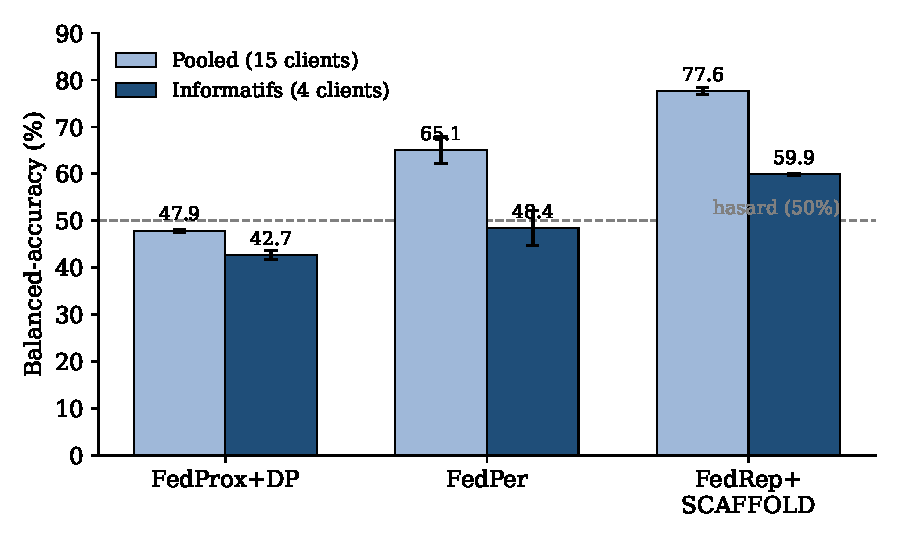
\includegraphics[width=0.8\linewidth]{fig_perso_comparison.pdf}
\caption{Balanced-accuracy of the three architectures, pooled metric (15 clients)
versus the metric restricted to the 4 informative clients. The gap between the two
bars of each pair is exactly the inflation caused by the single-class clients
(Section~\ref{sec:method}).}
\label{fig:perso}
\end{figure}

On the informative clients, the hierarchy FedProx+DP $<$ FedPer $<$ FedRep+SCAFFOLD
is statistically clear ($p<10^{-7}$ for all three pairwise comparisons), visible at a
glance in Figure~\ref{fig:perso}, where the gap between the two bars of each pair
directly measures how much the pooled metric overstates real performance. FedPer's
gain (+5.7 points versus FedProx+DP) is solid but markedly more modest than the
apparent inflation on the pooled metric (+17.2 points); raw accuracy also improves,
but marginally ($+0.95$ point, $p=0.04$). FedRep+SCAFFOLD goes further (+17.2 points
versus FedProx+DP on the informative clients) and is markedly more stable (standard
deviation 0.22 versus 3.65 for FedPer), at the cost of a $\approx5\times$ higher
compute cost and an unresolved confound (a 2-layer head \emph{and} SCAFFOLD change
simultaneously relative to FedPer).

\textbf{FedPer and FedProx differ along two axes}: the duration of personalization
(30 continuous rounds versus 8 epochs of post-hoc fine-tuning) and granularity (head
only versus the entire network). A dedicated test, isolating these two factors from
the same starting checkpoint and with re-seeded fine-tuning (5 seeds, paired $t$-test),
shows that \textbf{granularity dominates by far} ($+7.4$ points at 8 epochs, $+6.5$
points at 30 epochs, $p<0.03$): personalizing only the head clearly outperforms
fine-tuning the entire network. \textbf{Duration also matters, but far more
modestly} ($+1$ to $+2$ points, $p<0.02$). Notably, a simple fine-tuning of the head
alone on the already-trained standard FedProx+DP checkpoint reaches
$55.88\pm2.35\,\%$, \textbf{more than FedPer itself}, with no dedicated architecture
and no associated deployment constraint.

A Bonferroni correction for these 4 simultaneous comparisons (adjusted threshold
$\alpha=0.05/4=0.0125$) shows that 3 of the 4 effects survive it: only granularity at
30 epochs ($p=0.0219$) no longer passes this stricter threshold, a weakening
mechanically tied to the fact that the duration effect itself narrows the granularity
gap at 30 epochs (the two networks converge with more training). The paired Wilcoxon
test, in addition, plateaus at $p=0.0625$ in all four cases: a floor artifact specific
to $n=5$ pairs whose differences all share the same sign ($2\times(1/2)^5$, the
minimum $p$-value attainable with so few seeds), not a sign of doubtful significance;
the $t$-test remains the appropriate read here.

\subsection{Quantization and Privacy}

INT8 quantization occurs with almost no loss under FL ($\approx-0.05\,\%$ error,
versus $0.52\pm0.65\,\%$ under the centralized model): DP-SGD's gradient clipping
($C=1.0$) acts as an implicit Tikhonov-style regularization (\textit{weight decay})
that sharply compresses the dynamic range of the weights (Table~\ref{tab:dynrange}),
spreading them more uniformly across the 256-level quantization grid and limiting the
saturation/resolution loss suffered by the centralized model, whose much wider dynamic
range is more heavily truncated by quantization.

\begin{table}[h!]
\centering
\small
\caption{Dynamic range of the weights ($\max(|w|)-\min(|w|)$, mean$\pm$std over
5 seeds) by training mode and noise level.}
\label{tab:dynrange}
\begin{tabular}{lcc}
\toprule
Configuration & Global dynamic range & \texttt{fc1.weight} dynamic range \\
\midrule
Centralized (global std.)  & $9.4467\pm1.0336$ & $7.1129\pm0.5652$ \\
FL+DP ($\sigma=0.6$)        & $2.9734\pm0.2251$ & $0.8979\pm0.0547$ \\
FL+DP ($\sigma=0.8$)        & $3.3718\pm0.1742$ & $0.9616\pm0.0701$ \\
FL+DP ($\sigma=1.8$)        & $3.0734\pm0.3360$ & $1.4376\pm0.1326$ \\
\bottomrule
\end{tabular}
\end{table}

\paragraph{Why does peak RAM vary with the noise level?} Table~\ref{tab:ram} details
memory usage measured just before and during Opacus's \texttt{get\_epsilon()} call,
as a function of $\sigma$. Outside of this call, the footprint specific to local
training remains stable and low ($\approx0.18$~MB) regardless of noise level; the
Opacus objects (engine, optimizer, \textit{dataloader}) are instantiated once per
client at the first round and reused thereafter. The peak during
\texttt{get\_epsilon()}, in contrast, grows sharply as $\sigma$ decreases: the PRV
(\textit{Privacy Random Variable}) accountant performs a numerical evaluation of the
accumulated privacy-loss distribution, and the smaller $\sigma$ is, the more
concentrated this distribution becomes; to maintain numerical precision during
integration, the algorithm then generates a much denser temporary numerical grid,
proportional to $1/\sigma$, which dominates the observed RAM peak.

\begin{table}[h!]
\centering
\small
\caption{Peak RAM (MB, mean$\pm$std over 5 seeds) at round 30, before and during the
privacy computation.}
\label{tab:ram}
\begin{tabular}{ccc}
\toprule
$\sigma$ & Before \texttt{get\_epsilon()} & During \texttt{get\_epsilon()} \\
\midrule
0.6 & $0.18\pm0.00$~MB & $33.65\pm3.30$~MB \\
0.8 & $0.18\pm0.00$~MB & $20.48\pm1.50$~MB \\
1.0 & $0.18\pm0.00$~MB & $16.05\pm1.70$~MB \\
1.4 & $0.18\pm0.00$~MB & $13.44\pm1.00$~MB \\
1.8 & $0.37\pm0.42$~MB$^{*}$ & $11.34\pm0.43$~MB \\
\bottomrule
\end{tabular}

\vspace{2pt}
{\footnotesize $^{*}$4 of the 5 seeds give $\approx0.18$~MB; a single one produces an
isolated value of $1.11$~MB, pulling the average up: most likely a one-off
measurement artifact rather than a real effect of $\sigma$.}
\end{table}

\section{Synthesis}

\subsection{Summary}

This work arrives at a result more fundamental than the FL-vs-centralized comparison
that was its starting point:

\begin{enumerate}[leftmargin=1.2em]
\item \textbf{Extreme heterogeneity across nurses limits the generalization of every
architecture tested}, centralized included: restricted to the 4 genuinely informative
clients, the centralized model collapses too (balanced-accuracy $45.73\,\%$, AUC
$0.267$, below chance).
\item This work provides a formal $(\varepsilon,\delta)$-DP guarantee~\cite{dwork2014foundations}
($\varepsilon=0.54\pm0.04$ at $\sigma=1.8$, below the commonly used threshold
$\varepsilon=1$) and honestly quantifies its cost: 10 points of balanced-accuracy on
the pooled metric, reduced to 3 points on the informative clients, for a statistically
equivalent raw accuracy.
\item This cost is attributable mostly to \textbf{decentralization}, not to privacy
(Section~\ref{sec:results}), and remains stable across the entire noise range tested.
\item A model deployable in 5.32~KB (FP32), quantizable to INT8 with almost no loss.
\item Architectural personalization (FedPer, then FedRep+SCAFFOLD) significantly
reduces the residual gap (48.4~\% then 59.9~\% balanced-accuracy on the informative
clients) without ever eliminating it, consistent with finding (1) that the underlying
problem is heterogeneity itself, not just the choice of architecture.
\item Most directly actionable result: a simple post-hoc fine-tuning of the
classification head (frozen extractor) on the already-trained standard FedProx+DP
checkpoint is enough to obtain most of the personalization gain, at a markedly lower
engineering cost than FedPer or FedRep+SCAFFOLD.
\end{enumerate}

\subsection{Limitations and Future Work}

\begin{itemize}
\item \textbf{Statistical scope}: the significance measured on the informative
clients rests on only 4 clients with a mixed test set, solid on this specific
dataset, not yet generalized to a 5\textsuperscript{th} population.
\item \textbf{$\delta$ slightly above the recommended threshold}: with
$n=306{,}886$ training windows, $\delta=10^{-5}$ now exceeds the usual threshold
$\delta<1/n$ by a factor of $\approx3$; a $\delta=10^{-6}$ would be recommended for a
future iteration.
\item \textbf{Unreliable INT8 size measurement}: \texttt{model.parameters()} does not
cover the weights packed by dynamic quantization; only the theoretical factor
($\times3.8$) is reported.
\item \textbf{Single-node simulation} (Flower): a real decentralized deployment on
physical wearables remains to be validated.
\item \textbf{Cost of decentralization not yet reduced}: weighted loss brought no
gain; reweighting the aggregation, more informative features, and stronger
personalization remain to be explored. A targeted lead: the optimal decision
threshold after local adaptation diverges in opposite directions depending on the
client, suggesting that \emph{per-client} threshold calibration could bring a recall
gain without modifying the model itself.
\item \textbf{Results specific to this dataset and this architecture}: should not be
generalized without validation on other datasets and model sizes.
\end{itemize}

\bigskip
\noindent{\footnotesize This document is a condensed version of the full report,
which additionally details: the complete per-client diagnostic of AUC-ROC and
confident-error concentration, the detailed architectures (full FedProx/DP-SGD/SCAFFOLD
formulas, the FedRep+SCAFFOLD training incident and its fix), as well as the full
trace of every numerical verification performed before publication
(\texttt{resultsfeat/audit\_final.md}).}

\printbibliography

\end{document}
